\documentclass[tikz,border=3pt]{standalone}
\usepackage[utf8]{inputenc}
\usepackage[T1]{fontenc}
\usepackage{lmodern}
\renewcommand{\familydefault}{\sfdefault}
\usepackage{sansmath}\sansmath
\usepackage{chemfig}
\usepackage{pgfplots}\pgfplotsset{compat=1.18,/pgf/number format/use comma,/pgf/number format/1000 sep={.}}
\usetikzlibrary{arrows.meta,calc,positioning,decorations.pathmorphing,patterns}
% paleta del sitio
\definecolor{nar}{HTML}{E8680C}\definecolor{narc}{HTML}{FFB35C}\definecolor{hielo}{HTML}{FFF3E8}
\definecolor{tinta}{HTML}{1D1D1F}\definecolor{gris}{HTML}{6E6E73}\definecolor{lila}{HTML}{7C5CF0}
\definecolor{azul}{HTML}{2F6FD6}\definecolor{menta}{HTML}{17A673}\definecolor{coral}{HTML}{E8342A}
\begin{document}
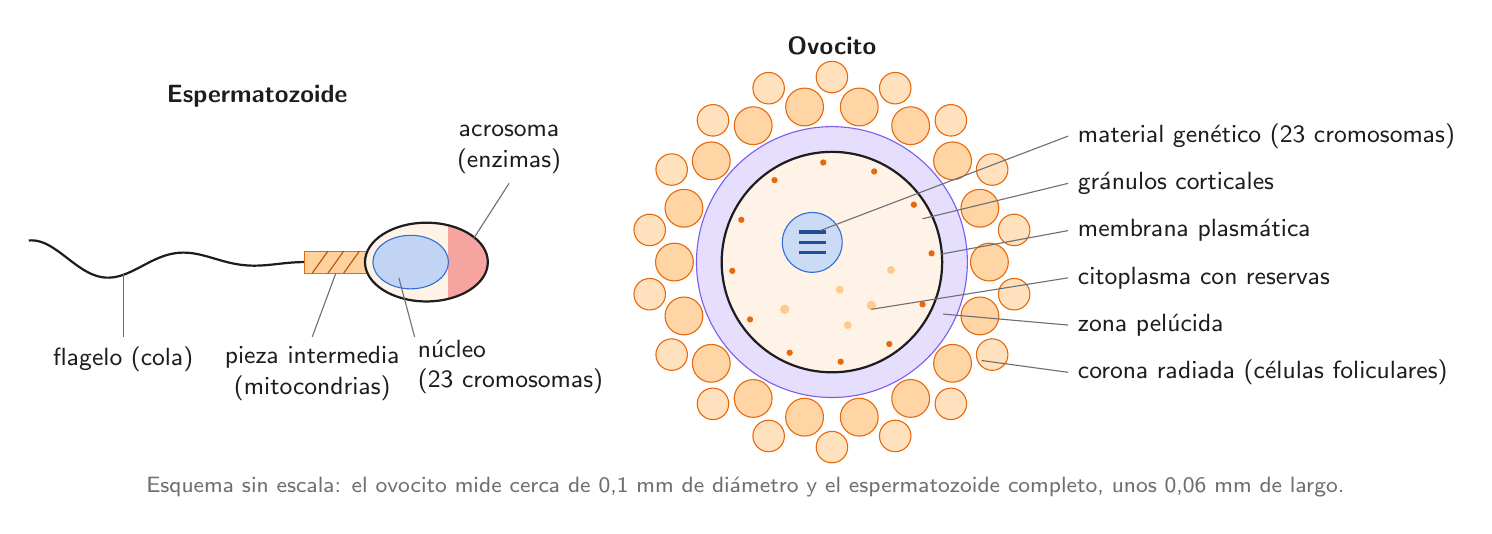
\begin{tikzpicture}[font=\small]
% ---- espermatozoide
\node[font=\small\bfseries,text=tinta] at (0.3,2.1) {Espermatozoide};
\draw[tinta,thick] plot[domain=-2.6:0.9,samples=90,smooth] (\x,{0.28*sin(deg(3.2*(\x-0.9)))*(0.9-\x)/3.5});
\draw[nar,fill=narc!60] (0.9,-0.14) rectangle (1.7,0.14);
\foreach \x in {1.0,1.2,1.4} \draw[nar!80!black] (\x,-0.14) -- (\x+0.2,0.14);
\begin{scope}
\clip (2.45,0) ellipse (0.78 and 0.5);
\fill[hielo] (1.6,-0.6) rectangle (3.3,0.6);
\fill[coral!45] (2.72,-0.6) rectangle (3.3,0.6);
\end{scope}
\draw[tinta,thick] (2.45,0) ellipse (0.78 and 0.5);
\draw[azul,fill=azul!30] (2.25,0) ellipse (0.48 and 0.34);
\draw[gris] (3.05,0.3) -- (3.5,1.0) node[anchor=south,text=tinta,align=center] {acrosoma\\(enzimas)};
\draw[gris] (2.1,-0.2) -- (2.3,-0.95) node[anchor=north west,text=tinta,align=left,inner sep=1pt] {núcleo\\(23 cromosomas)};
\draw[gris] (1.3,-0.14) -- (1.0,-0.95) node[anchor=north,text=tinta,align=center] {pieza intermedia\\(mitocondrias)};
\draw[gris] (-1.4,-0.15) -- (-1.4,-0.95) node[anchor=north,text=tinta] {flagelo (cola)};
% ---- ovocito
\begin{scope}[shift={(7.6,0)}]
\node[font=\small\bfseries,text=tinta] at (0,2.75) {Ovocito};
\foreach \a in {0,20,...,340}{\draw[nar,fill=narc!55] (\a:2.0) circle (0.24);}
\foreach \a in {10,30,...,350}{\draw[nar,fill=narc!40] (\a:2.35) circle (0.2);}
\draw[lila,fill=lila!20] (0,0) circle (1.72);
\draw[tinta,thick,fill=hielo] (0,0) circle (1.4);
\foreach \a in {5,35,...,355}{\fill[nar] (\a:1.27) circle (0.04);}
\draw[azul,fill=azul!25] (-0.25,0.25) circle (0.38);
\foreach \y in {0.12,0.25,0.38}{\draw[azul!70!black,line width=1.2pt] (-0.42,\y) -- (-0.08,\y);}
\fill[narc!70] (0.5,-0.55) circle (0.06) (0.2,-0.8) circle (0.05) (0.75,-0.1) circle (0.05) (-0.6,-0.6) circle (0.06) (0.1,-0.35) circle (0.05);
\end{scope}
\draw[gris] (7.45,0.4) -- (10.6,1.6) node[anchor=west,text=tinta] {material genético (23 cromosomas)};
\draw[gris] (8.75,0.55) -- (10.6,1.0) node[anchor=west,text=tinta] {gránulos corticales};
\draw[gris] (8.98,0.1) -- (10.6,0.4) node[anchor=west,text=tinta] {membrana plasmática};
\draw[gris] (8.1,-0.6) -- (10.6,-0.2) node[anchor=west,text=tinta] {citoplasma con reservas};
\draw[gris] (9.01,-0.66) -- (10.6,-0.8) node[anchor=west,text=tinta] {zona pelúcida};
\draw[gris] (9.5,-1.25) -- (10.6,-1.4) node[anchor=west,text=tinta] {corona radiada (células foliculares)};
\node[text=gris,font=\footnotesize,align=center] at (6.5,-2.85) {Esquema sin escala: el ovocito mide cerca de 0,1 mm de diámetro y el espermatozoide completo, unos 0,06 mm de largo.};
\end{tikzpicture}
\end{document}
